\documentclass[12pt,a4paper]{article}
\usepackage{times}
\usepackage{durhampaper}
\usepackage{harvard}
\usepackage{underscore}
\usepackage{graphicx}
\usepackage{url}
\usepackage{hyperref}
\usepackage[subtle]{savetrees}
\usepackage[ruled,vlined,linesnumbered]{algorithm2e}

%\package save trees - to save room

\citationmode{abbr}
\bibliographystyle{agsm}

\title{Procedural World Building in Roguelike Games}
\author{Benjamin Jones}
\student{Benjamin Jones}
\supervisor{Dr. Tom Friedetzky}
\degree{MSci Natural Sciences}


\begin{document}

\maketitle

\begin{abstract}

{\bf Context/Background}

Procedural content generation in videogames has seen a surge in popularity in recent years. However as game development progress, users expect more and more intelligent and engaging game level design and as a result, investigating new, interesting methods of procedural content generation is vital to keeping end users happy.

{\bf Aims}

This project aims to draw comparisons between current methods of procedural content generation in a roguelike game environment and build upon them to create different and exciting methods of level design. The implementation will focus on creating a number of novel algorithms alongside an intelligent method of evaluating their suitability. 

{\bf Method}

A variety of algorithms will be developed and implemented by building on and combining various existing methods found in existing roguelikes and more sophisticated modern games. Perlin and Simplex noise algorithms will be used to generate the initial random seed, which will then be modified by a variety of methods including the Cellular Automata approach and the use of geometric space-filling curves such as the Hilbert curve and Sierpinski curve. The effectiveness of these will then be evaluated by a custom heuristic, ensuring the quality of the resulting world. 

{\bf Proposed Solution}

The proposed game will be built and played in Java using the JFrame and asciipanel libraries as a framework. The combination of existing algorithms and novel techniques will produce multiple potential procedurally generated worlds, which will be evaluated by the program and the best fit will form the playable environment in a roguelike game. 

\end{abstract}

\begin{keywords}
Procedural content generation, roguelike, world building, noise algorithms, artificial intelligence, heuristic, space-filling algorithms.
\end{keywords}

\section{Introduction}
\subsection{Roguelike Games} \label{ssec:rogue}


The term Roguelike stems from the original 1980s UNIX dungeon crawler `Rogue' created by Michael Toy and Glenn Wichman, giving birth to hundreds of games such as Nethack and Angband that follow the same style and structure and revolutionising the gaming industry as we know it today \cite{Dunhack}. There are many different styles of roguelikes these days, but most share the same core features: turn-based gameplay, procedurally generated tile-based dungeons and randomly created monsters and items \cite{pgcbook}. 

The basic premise of the game has the player controlling a single character through numerous ASCII represented dungeons filled with items, monsters and traps. However what made it so unique and revolutionary at the time was the fact that the game was different every time you played it thanks to its procedurally generated nature \cite{roguebasin}. 



\subsection{Procedural Content Generation} \label{ssec:PCG}

Procedural content generation (PCG) is the process of creating content through the use of random numbers as seeds to generate objects using code and mathematical functions, as opposed to the typical method of being manually created by a developer \cite{pgcbook}. This has many possible applications, from running real-world simulations on procedurally generated objects and environments \cite{vast}, to generating interesting and unique textures and graphics \cite{imagesynth}, and of course for use in video games. This is typically achieved by modifying the results of mathematical noise algorithms \cite{pgcbookch4}, which generate heightmaps and intensity maps that can be transformed into random terrains. \\

Procedural generation has many advantages unrivalled by other generation methods: it is typically much faster to evaluate, it can generate arbitrarily complex and intricate designs on the fly and has particularly low memory footprint \cite{surveyPNF}. Additionally, the variation of input parameters can easily generate an incredible number of uniquely styled designs. The result is that procedurally generated game content has the capability to offer every game user a unique gaming experience every time they play. \\

% ref paper \cite{surveyPNF}
% %Procedural noise has many advantages: it is typically very
% fast to evaluate, often allowing evaluation of complex and
% intricate patterns on-the-fly, and it has a very low memory
% footprint, making it an ideal candidate for compactly generating
% complex visual detail. In addition, with a suitable set of
% parameters, procedural noise can be used to easily generate a
% large number of different patterns. Finally, procedural noise
% is often randomly accessible, so that it can be evaluated independently
% at every point in constant time.

A perfect example of the power and potential of PCG is \emph{Minecraft}. At the time of writing, Minecraft sales have hit more than 70 million world-wide, making it one of the most popular games of all time \cite{ukie}. However at it's base, Minecraft draws many parallels with the methods of generation seen in even some of the earliest Roguelike games, for example, Minecraft uses at it's core a 3D adaptation of the 2D Perlin noise algorithm adopted by many popular roguelikes \cite{notch}, including \emph{Nethack} and \emph{Dwarf Fortress} \cite{Dunhack}.\\

Also recently hitting the spotlights recently is indie game \emph{`No Man's Sky'}, a futuristic sci-fi role-playing game (RPG) that procedurally generates an entire galaxy populated with up to 18 quintillion planets for the player to explore at their leisure. Developed by a team of only 10 people, No Man's Sky demonstrates the power and potential that procedural generation has to offer to the gaming market. \\

A final game worth mentioning is award-winning 2004 German 3D shooter `\emph{.kkrieger}'. The game won its award not because of its content however, but because its extensive use of procedural generation techniques mean everything from the textures to the in-game sounds (as well as the traditional monsters and levels) are generated completely procedurally. This allows the entire game to be coded in just 96 kilobytes of memory, meaning that even screenshots of the game take up more room than the game itself and allowing .kkrieger to take up to 3000x less storage than an equivalent conventionally designed game \cite{kkrieger}. This game exemplifies what can be achieved using procedural techniques.\\

As games get more complex and take longer to build, coming up with new and exciting ways to programatically generate game content could be the key to a revolution in the gaming industry (expected to reach \$103bn in 2017 \cite{newzoo}).




% \subsection{Evaluation of Literature}

% DRAFT PARAGRAPH
% In a project such as this, it is important to note that the amount of academic research in this area is limited and (one presumes) much of it is being undertaken by private game companies 
% A lot of the current research and experimentation is being undertaken by bloggers and home enthusiasts


\subsection{Project Aims}

The purpose of the project in summary is to investigate the various ways procedural generation is used to generate game environments, and then design and build one or more variants based on the best of these approaches with the aim to create exciting, interesting and challenging environments for a roguelike game setting. The project will also aim to evaluate the output of the algorithms with a fitness heuristic function to identify whether or not a generated output meets these aims. \\

The deliverable should be an executable program running in the Java programming language that is capable of producing two dimensional ASCII worlds for a player to explore. The algorithm should be deterministic, and ideally will be efficient such that it is capable of producing and evaluating multiple worlds quickly, identifying the best and putting that forward to the playable game environment. The game world should have the additional constraint that all parts of the map should be traversable from any other part of the map, explicitly checked by the algorithm. 
%any other constraints



%introduction still needs: Perlin noise, Cellular Automata, maze generation and puzzle generation.  

\subsection{Deliverables}


Please note: unfamiliar concepts introduced here will be discussed later in the design section.

\textbf{Minimum objectives:}

\begin{itemize}%\itemsep0pt

	\item Produce a basic game engine in Java to handle user input and ASCII grid output, to enable world creation and character movement, including side scrolling.
	\item Choose appropriate data structures.
	\item Implement a deterministic 2D noise generator to produce fundamental basis for procedural dungeon creation.
	\item Implement a smoothing function based on the Cellular Automata approach to produce a basis for a cave-like structure.
	\item Implement a probability density field for the placement of walls and floor based upon a mathematical space filling function and a noise generator. 
\end{itemize}
\textbf{Intermediate objectives:}
\begin{itemize}
	\item Develop probability density algorithm to produce interesting and varied worlds based upon various mathematical functions.
	\item Produce a metadata structure for the world that has extra information about each grid space, including items and other features.
	\item Look at potential effects of using more complex noise algorithms (eg Perlin \& Simplex) in world creation.
	\item Be able to check that a world is connected.
\end{itemize}
\textbf{Advanced objectives:}
\begin{itemize}
	
	\item Develop world evaluation heuristic capable of rating worlds on a number of criteria.
	\item Look into maze generation algorithms and underlay them in the world.
	\item Investigate possibility of procedurally generated dungeon `puzzle' rooms.
	\item Optimisation of procedural generation techniques such that generation is fast enough to quickly generate multiple worlds and select the most suitable using the world evaluation heuristic. 
\end{itemize}


\section{Design}

\subsection{Requirements}

\begin{table}[h!]
\centering
\begin{tabular}{l|l|l}
\textbf{ID}  & \textbf{Requirement}                                           & \textbf{Priority} \\ \hline
FR1 & Implementation of fundamental game engine in Java handling IO    & High     \\
FR2 & Implementation of rudimentary noise algorithm                         & High     \\
FR3 & Create Cellular Automata style algorithm for noise smoothing     & High     \\
FR4 & Create probability density algorithm to determine block identity & High     \\
FR5 & Created worlds must have the connected property    			   & Medium    \\
FR6 & Produce metadata structure for grid space                        & Medium   \\
FR7 & Produce world fitness heuristic                                  & Medium  \\ \hline
% \end{tabular}
% \end{table}

% \begin{table}
% \centering
% \begin{tabular}{l|l|l}
% ID  & Non-Functional Requirement                                           & Priority \\ 
% \hline
NFR1 & Optimisation of space filling function in probability density algorithm    & Medium    \\
NFR2 & Improvement of noise algorithm using Perlin approach & High \\
NFR3 & Ability to produce interesting worlds with definable features & High \\
NFR4 & Ability to test for world connectivity            & Medium     \\
NFR5 & Additional game areas involving maze/puzzle generation & Low \\  

\end{tabular}
\caption{Functional \& Non-Functional Requirements}

\label{table:1}
\end{table}

\subsection{Specification of Software}

The implementation of the project will be achieved in Java (SE 1.8). There are a number of reasons why Java is well suited to this project. Java is a well established, high-level language used by millions of people all over the world and as such there are many previous implementations and libraries specific to Roguelikes in Java from which the project can benefit. By utilising copyright free libraries and examples from previous roguelike enthusiasts, a quick framework for the game engine can be easily created and ammended to the project's aims, while focussing development on more important and interesting aspects of the implementation. To this extent, many suitable libraries exist. In particular, we will make extensive use of the `JFrame' and `asciipanel' libraries. The former is a well known library enabling the use of a windowed frame for which the program is able to handle input and output, and the latter a `Java Console System Interface', which is popular among roguelikes and allows for ASCII text character output in various colours. \\

Java is also particularly useful due to its highly object-orientated nature. Since the design aspect of the game can be separated into many parts, it is helpful to be able to abstract and separate each process into different classes, allowing the main focus of the algorithmic side of the project to be apart from the engine handling input and output to the console. This makes development much easier, as well as improving bug fixing and code readability.\\

In addition, Java is known as a platform-neutral language \cite{java}, meaning the final implementation will be easily run on almost any platform (except mobile) without the need to recompile the source. This is very powerful and makes it easy to continue development and evaluation from a variety of computers during the project, especially in the event that additional processing power is preferred later on to run and evaluate multiple simulations of the design algorithms. [POTENTIALLY REMOVE PARAGRAPH] \\

Finally, Java has been chosen because of its familiarity. While the project may benefit from features of other languages (such as the rapid prototyping and clear code of Python), familiarity with Java enables a reduced implementation period in the system development life cycle, allowing more time to be spent on the design, planning and evaluation aspects of the cycle. 
\\

The `Agile' software development approach will be used in the project in order to meet its aims. This is because the project will benefit from achieving each functional target in individual rapid sprint cycles, which can then be thoroughly tested for quality between cycles before the next implementation aspect is introduced. This also enables a higher degree of freedom than other software development approaches (such as the `Waterfall' approach), enabling the constant evaluation and possible change of separate requirements should the fulfillment of previous ones require so, due to the unpredictable nature of certain algorithms effectiveness and ease of implementation.


\subsection{System Design}

The game engine that houses the game world and handles input and output as mentioned will primarily use the asciipanel library, but also follow from an open source implementation created by an online roguelike programmer known as `Trystan' \cite{trystan}. This provides a framework that is able to be modified for the purposes of this project, in order to focus on more complex aspects of the procedural generation algorithmic design. The capabilities of the resulting game engine allow for an interactive window of a similar quality to that of estabilished roguelikes such as Nethack and even Dwarf Fortress. 


% \begin{figure}[h]
% \begin{minipage}{.5\textwidth}
%   \centering
%  	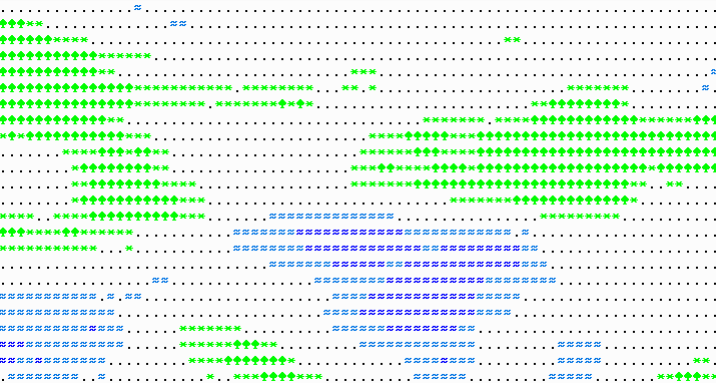
\includegraphics[width=6.25cm,height=4cm]{images/asciipanel1inv.png}
% 	\caption[]{Asciipanel GUI example \\ Image sourced from: \\\url{http://www.headchant.com/2012/02/15/asciipanel-as/}}
% 	\label{fig:fig1}
% \end{minipage}
% \begin{minipage}{.5\textwidth}
%   \centering
%   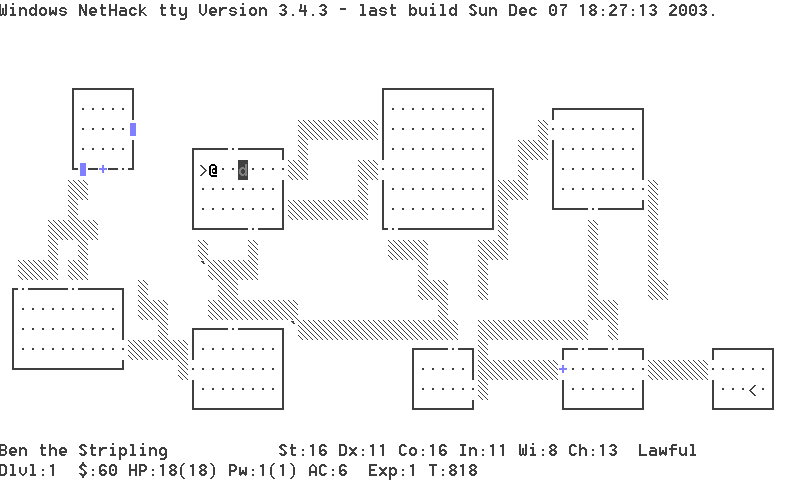
\includegraphics[width=6.25cm, height=4cm]{images/nethack2.png}
%   \caption[]{Nethack GUI example [probably copyright]}
%   \label{fig:fig2}
% \end{minipage}
% \end{figure}

\begin{figure}
\centering
 	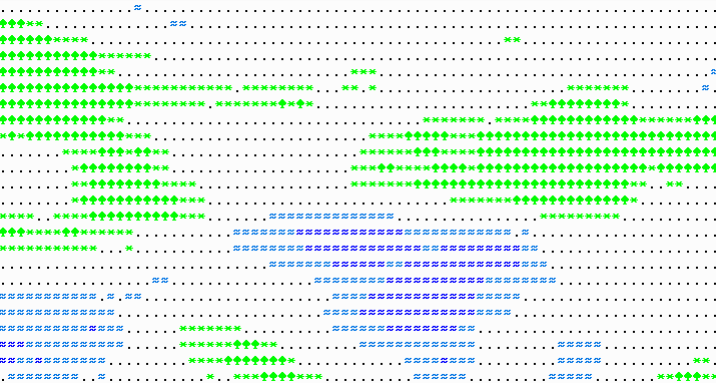
\includegraphics[width=6.25cm,height=4cm]{images/asciipanel1inv.png}
	\caption[]{Asciipanel GUI example. Image sourced from: \url{http://www.headchant.com/2012/02/15/asciipanel-as/}}
	\label{fig:fig1}
	\vspace{2ex}
	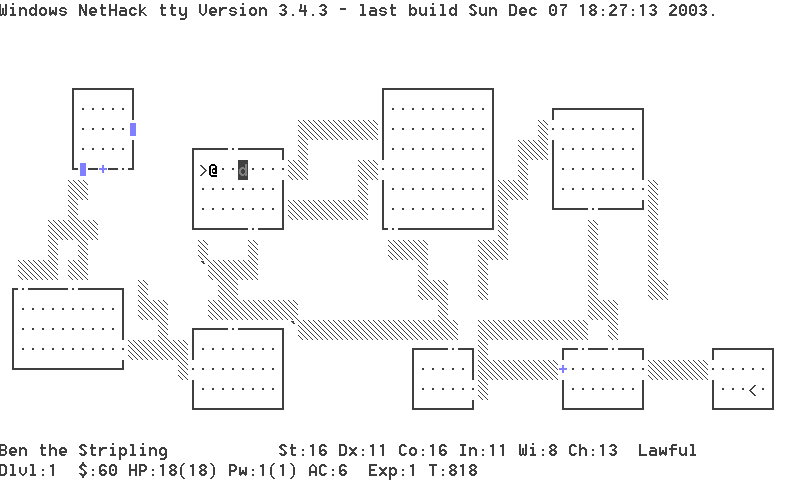
\includegraphics[width=6.25cm, height=4cm]{images/nethack2.png}
  \caption[]{Nethack GUI example}
  \label{fig:fig2}
 \end{figure}



\subsection{Noise and Smoothing Algorithms}
\label{subsec:noise}

Noise algorithms are crucial to most procedurally generated content and will feature heavily in the project as they form the foundation for the world. The noise environment can then be moulded by a number of different approaches to form the basis of the map. \\

There are a few kinds of noise algorithm, from very basic noise algorithms where each `pixel' has an equal chance to be filled or unfilled, to much more advanced versions such as Perlin noise and Simplex noise \cite{textmodel}\cite{improvepnoise}. The type of noise algorithm selected depends on the project requirements, and the sort of algorithm that will aim to transform the noise environment into a playable, enjoyable world. 

% The psuedocode for a basic binary noise algorithm described in FR2 (Table:\ref{table:1}) is shown in algorithm \ref{Alg:alg1} below:

% \begin{algorithm}
% 	\For{$x$ \textless $map width$}{
% 		\For{$y$ \textless  $map height$}{
% 			\If{$tile[x][y]$= psuedo_random_number() \textless 0.5}{
% 				$tile[x][y]$ = $floor$
% 			}
% 			\Else{
% 				$tile[x][y]$ = $wall$
% 			}
% 		}
% 	}
% 	\caption{Basic binary noise production}
% 	\label{Alg:alg1}
% \end{algorithm}
% % 
% not necessary 

\subsection{Cellular Automata}

The binary noise algorithm is simple and easy to implement, paving the foundation for a smoothing technique known as `Cellular Automata'. This technique became famous in the 1970's when British mathematician John Horton Conway devised his evolutionary `Game of Life', a game that transforms an initial state of `cells' into intricate and interesting patterns and designs by the use of 4 rules \cite{cellauto}: 

\begin{itemize}
	\item Survivals: Every cell with two or three neighbouring cells survives for the next generation.
	\item Deaths. Each cell with four or more neighbours dies (is removed) from overpopulation. Every cell with one neighbor or none dies from isolation.
	\item Births. Each empty cell adjacent to exactly three neighbours--no more, no fewer--is a birth cell. A cell is placed on it at the next move.
\end{itemize}

This process is used upon the result of the binary noise algorithm to `smooth' out the landscape by turning areas that are mostly neighbouring walls into walls and areas mostly neighbouring floors into floors. The process is then repeated a number of times until the desired combination of walls and floors is achieved. \\

% An example of the process run on the basic noise algorithm seen in algorithm \ref{Alg:alg1} is shown below:

\begin{figure}[h]
  \centering
 	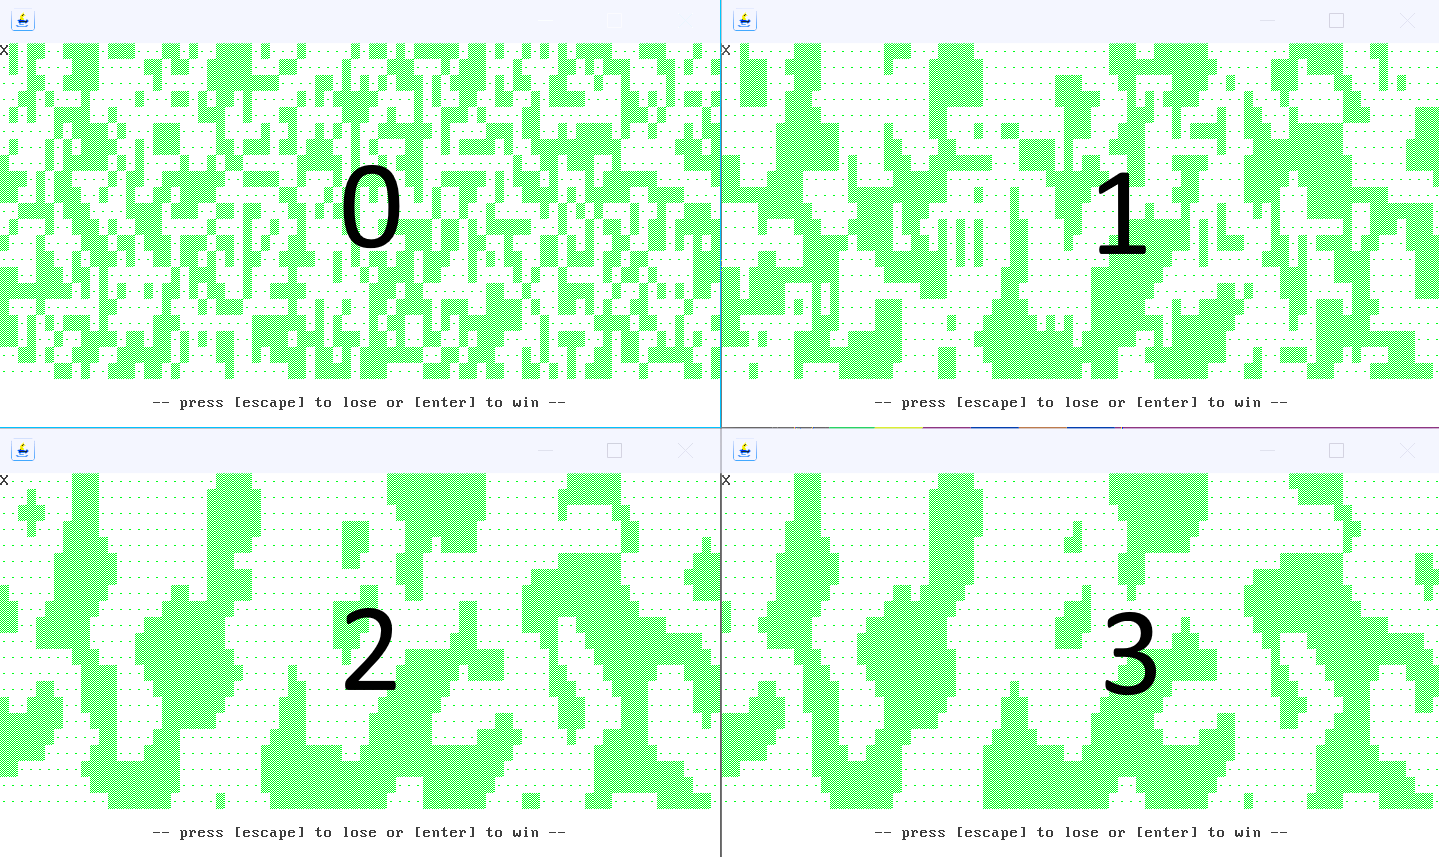
\includegraphics[scale=0.5]{images/cellauto.png}
	\caption[]{Cellular Automata cave smoothing. The numbers indicate the iterations of the algorithm, where the top-left image is before the smoothing process}
	\label{fig:fig3}
\end{figure}

It's clear to see from figure \ref{fig:fig3} that this process very quickly converges to produce interesting, procedurally generated cave-like structures for a roguelike game setting, in addition to being computationally inexpensive (the generation is instantaneous even for very high levels of iterations (1000+) on a moderately powerful machine). \\

It is, however, limited in its usefulness by itself, as the results of the algorithm are inconsistent, occasionally producing uninteresting or unnatural worlds. Worse still, its particularly prone to what is known as `the isolated cave problem', whereby produced maps are often `disconnected'- that is the player is unable to advance from any location to any other location. \\

This nature (seen in fig \ref{fig:fig3}) breaks functional requirement 5 of the project, and therefore alternative methods or amendments must be implemented to achieve this goal. There are a variety of ways that we may achieve this. One approach for example would be to generate many worlds and test for completeness, discarding the worlds that don't fit our criteria. Because of the instantaneous nature of this method of world population, we are able to create and evaluate many worlds very quickly, however the problem arises when we wish to expand our world size. A larger world boundary results in an increased statistical probability that the created world will be disjoint almost every time. An alternative approach would be to identify disjoint sections and connect them up by removing wall segments. This does guarantee connectivity, but is also prone to making the world look unnatural, defeating the point of using the algorithm in the first place. \\

One of the biggest advantages with Cellular Automata however is that rules can be tweaked easily to enhance the output. By experimenting with these rules, previous adopters of this approach have been able to produce vastly different environments, some of which are much less likely than others to form disjointed caves \cite{roguebasin}. \\


\subsection{Perlin Noise Algorithm}

The approach above is a good starting point for the project but even with the finest tweaking of the algorithms rules, the output is limited by its ability to only produce binary maps (only walls and floors) and its inability to create specific features or structures procedurally, falling short of our non-functional requirement 3. With this aim in mind, we look to a different noise producing algorithm, Perlin noise, to advance upon this requirement. \\


Perlin noise was developed by Ken Perlin in 1985 and has been widely used in applications ranging from procedural world generations to computer graphics \cite{imagesynth} \cite{surveyPNF}. It is particularly good for creating natural looking textures in games and simulated environments, and could be adapted for use in a roguelike setting.\\

It should be noted at this point that Perlin noise is not without flaws and Perlin himself noted a number of improvements on his original design in his 2002 paper, `Improving Noise' \cite{improvepnoise}. The result of his paper was the invention of `Simplex Noise', a superior noise algorithm with better efficiency, however Perlin noise is still useful because it is both simpler to implement and the effect of its inefficiencies are questionable in the scope of this project. The project aims to quantify these at a later date. \\

Perlin noise generation can be split into two components, a noise generating function, and an interpolation function. The noise generating function operates in a similar fashion to the binary noise generator described in section \ref{subsec:noise}, except instead of taking on either 0 or 1, the function generates floating point numbers between 0 and a maximum value (known as the amplitude). The interpolation function then smoothly averages across these values, as seen in figures \ref{fig:fig4} \& \ref{fig:fig5}, and we take the distance between points on the x-axis to be the wavelength of the noise wave \cite{Howuseperlin}. 


\begin{figure}[h!]
  \centering
 	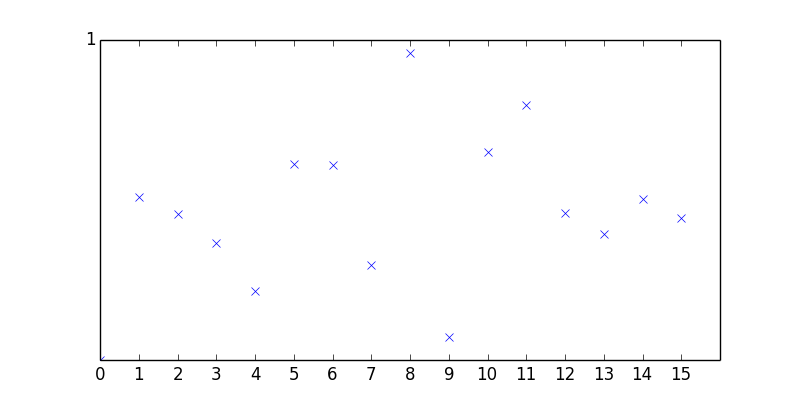
\includegraphics[scale=0.5]{images/figure2.png}
	\caption[]{Example 1-dimensional noise function. A random value with a maximum amplitude of 1 is assigned to each point on the X axis.}
	\label{fig:fig4}
\end{figure}

\begin{figure}
  \centering
 	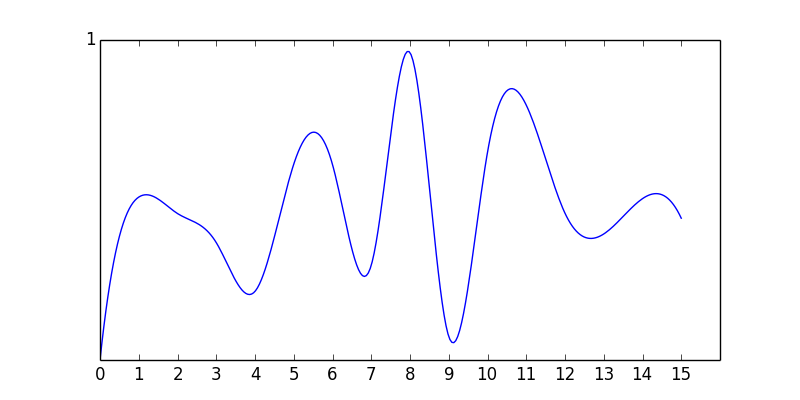
\includegraphics[scale=0.5]{images/figure1.png}
	\caption[]{By smoothly interpolating between the values, we obtain a continuous function, with wavelength 1.}
	\label{fig:fig5}
\end{figure}

To generate Perlin noise, we generate many of these waves (in 1 dimension) or images (in 2 dimensions) at varying wavelengths and frequencies (the combination of which is known as an octave), and sum them up to produce our final image. An example of the process may be seen in figure \ref{fig:fig6}.

\begin{figure}[h!]
  \centering
 	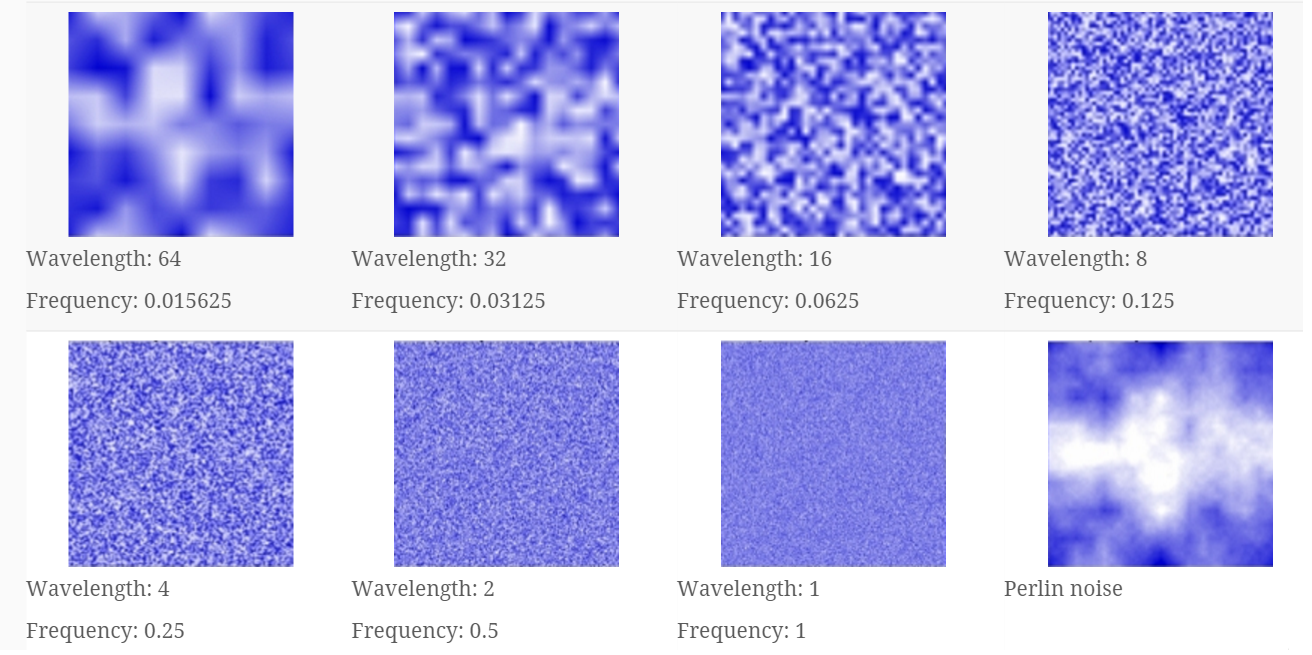
\includegraphics[scale=0.65]{images/perlingen.png}
	\caption[]{The Perlin noise generation process. The final image is the result of the previous 7 images summed together. Image taken from Tulleken. H, (2009), \emph{`How to Use Perlin Noise in Your Games'}, Dev.Mag, (20), sourced from: \url{http://devmag.org.za/2009/04/25/perlin-noise/} on 09/02/16}
	\label{fig:fig6}
\end{figure}

The applications of this are many-fold, but in a roguelike game this can be used to create the idea of depth into a 2-dimensional world, which was not possible using our previous Cellular Automata approach. The Perlin noise image may be used to form a height-map, where density is proportional to height. This allows the introduction of alternative tile types, such as hills, forests, trees and plains with different movement cost to the character, or even impassable objects such as canyons, crevasses or mountains. Such depth in the game adds considerable complexity, expanding on the many ways the game can already be played. An example can be seen in figure \ref{fig:fig7} below:

\begin{figure}[h!]
\begin{minipage}{.5\textwidth}
  	\centering
 	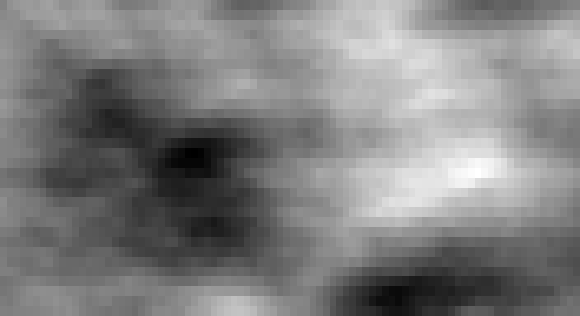
\includegraphics[width=6.25cm,height=4cm]{images/perlin2.png}
	\caption[]{Normalised grayscale fractal Perlin noise, sourced from \url{http://www.nolithius.com/game-development/world-generation-breakdown}}
	\label{fig:fig7}
	\end{minipage}
% \end{figure}
% \begin{figure}
	\begin{minipage}{.5\textwidth}
 	\centering
 	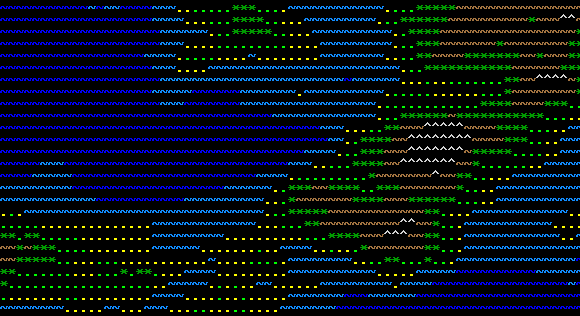
\includegraphics[width=6.25cm,height=4cm]{images/terrain.png}
	\caption[]{Terrain applied to Perlin noise from figure \ref{fig:fig7}. Sourced from \url{http://www.nolithius.com/game-development/world-generation-breakdown}}
	\label{fig:fig8}
\end{minipage}
\end{figure}

% use one figure one caption

\subsection{Space-Filling Curves}

The results of Perlin noise look promising, with interesting structures and added complexity introduced into the produced worlds. However it is clear that a structure to the world is still lacking, with no easily defined start or end point, specific features, rooms or obvious places to put monsters, traps and treasure that make a Roguelike game so special to play. This project aims to solve these problems by hybridising well-known noise algorithms such as Perlin noise with mathematical functions known as `space-filling curves', in a novel approach not yet seen to the best of our knowledge in previous Roguelikes.\\

Space-filling curves are fractal in nature, and given a starting seed, produce deterministic and characteristic curves, shapes and paths that will be used to form a basis for the world generation algorithm.\\

This will be achieved by taking random segments of a generated curve and overlaying them on top of a Perlin noise image. The result will become a `probability density heightmap' for the world, where densely populated regions will have a greater chance to become traversable tiles. The advantage of this is that the generated world will be much more likely to have a structure, with defining curves, edges and paths from one edge to another (potentially linking to other generated segments), while maintaining the natural look and feel of a Perlin generated environment. Additionally, there are a wealth of different types of space-filling curves; some examples are displayed below in figure \ref{fig:fig9}. The project will experiment with a number of these to determine the resulting output, and potentially use multiple ones to reflect upon different in-game environments or `biomes', with their own look and feel arising from the different structures provided by the various curves. \\

As an extension, it may be possible to fulfil non-functional requirement 5 by experimenting with a different set of mathematical algorithms: procedural maze generators. Depending on initial parameters, maze generators are able to procedurally produce a wide variety of shapes in a similar fashion to space filling curves, except they have a specified entrance and exit(s). However the purpose of a roguelike is not necessarily to solve a maze-like puzzle, and the usefulness over a regular space filling curve (when not taking the maze as a whole) is questionable.

\begin{figure}
\centering
	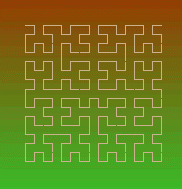
\includegraphics[width=4.5cm,height=4.5cm]{images/hilbert.png}
	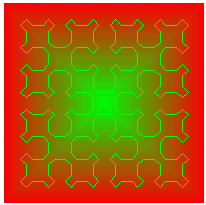
\includegraphics[width=4.5cm,height=4.5cm]{images/sierpinskicrv.png}
	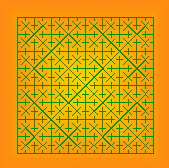
\includegraphics[width=4.5cm,height=4.5cm]{images/cesaro.png}
	\caption[]{\label{fig:fig9} Left: The Hilbert curve provides large, easy paths but is limited to just horizontal and vertical degrees of freedom. Middle: The Sierpinski curve doesn't produce easily followable channels, but could form the basis of several rooms for various gameplay features. Right: The Cesaro curve looks less natural but might provide interesting results for separate in-game biomes. All images sourced from TGMDev, available online at: \url{http://www.tgmdev.be/applications/acheron/acheron.php}	}
	
\end{figure}


\subsection{Evaluation}

The overarching aim of the project is to produce interesting and functional worlds. My evaluation therefore will be split into two sections, one for evaluating the level of interest in the world, and one for assessing the functionality of generated worlds. \\

In order to evaluate how interesting a world will be, the project will aim to use two methods. The first will be a simple user evaluation of created worlds. This may be in the form of simply noting down interesting aspects of multiple generated worlds, or in a more formal user feedback questionnaire. Importantly, the Agile approach to the development of this project allows repeated user evaluation to take place between development sprints, allowing feedback to be taken into account during the next phase. \\

Additionally, in-line with functional requirement 7, the project will aim to create a `fitness heuristic' that will identify key features of interesting maps; for example the presence of multiple pathways, narrow and unavoidable passage ways to put monsters, dead end rooms to put items and traps, and the ratio of traversable to non traversable terrain. This may also be modelled on the feedback from end users in the feedback questionnaire. The combination of fitness factors such as these will result in the return of a weighted world fitness coefficient, allowing the program to have some level of automative knowledge of how `interesting' a generated world is. While it is an important aspect of a roguelike for the world generation to be quick, there must be a trade-off between world quality and real-time terrain generation speed. Provided the world generating process is fast enough, the program would be able to generate multiple worlds and select the best to output to the game. \\

The functionality of worlds will be assessed by a world completeness algorithm, fulfilling non-functional requirement 4. The aim of this will be to test if a world is accessible from any one point a to any arbitrary other point b. While this is non-essential (it may not be necessary to access all parts of a generated world), it may also be game-breaking if large sections or progressions to the game are cut off by procedurally generated walls. Therefore, the algorithm will test for both circumstances: whether it's possible to access the exit point from the starting position, and then whether the entire world is `connected', and if not, measure exactly how connected it might be. A negative result of the former criterion results in the generated world being discarded immediately, while the latter must be reviewed in a user feedback questionnaire as to whether or not the world is still likely to be enjoyable, and to what extent. The algorithm may then be fine-tuned based on user feedback to keep or discard the worlds based on the results of user feedback. 




% could be utilised in our world environment. We will use this nature to 


% fractals curves exhibit a very interesting property known as self-similarity. If you observe precisely the details of a fractal curve, it appears that a portion of the curve replicates exactly the whole curve but on a different scale. Mathematicians have in fact created geometrical fractal curves long before the introduction of the fractal geometry by Benoit Mandelbrot. Some of these curves are well-known as the Von Koch's snowflake or the triangle of Sierpinsky. \\

% -probability density approach
% -probability of something being there or not
% -produces an underlying structure, making those pixels/tiles more likely to contain traversable spaces 
% -and other tiles more likely to not be traversable
% -with perlin noise filling in the rest
% -random sections of the space filling algorithm selected


% -different paths, checked for entrance and exits
% -possibility of expanding to maze generation over the top
% -guaranteed, reliable, deterministic and probabilistic, as well as procedural paths in our dungeon/world.


% % DEFINITELY include about testing and evaluating 
% % software engineering practices for testing and evaluating 
% % objective criteria evaluation, runtime etc
% % objective measures to do with quality of something
% % possibility as well- user based evaluation 
% % eg does it feel how you'd like it to feel? use questionnaire
% % 1/3 of a page is achievable 
% % k connectivity- ways of travelling 
% % diameter 
% % heuristic for evaluation- get the player to play the best weighted average 







% \subsection{Main Text}

% The font used for the main text should be Times New Roman (Times) and the font size should be 12.  \textbf{The first line of all paragraphs should be indented by 0.25in, \emph{except} for the first paragraph of each section, subsection, subsubsection etc.} (the paragraph immediately after the header) where no indentation is needed.

% % use \noindent

% \subsection{Figures and Tables}
% In general, figures and tables should not appear before they are cited.  Place figure captions below the figures; place table titles above the tables.  If your figure has two parts, for example, include the labels ``(a)'' and ``(b)'' as part of the artwork.  Please verify that figures and tables you mention in the text actually exist.  make sure that all tables and figures are numbered as shown in Table  and Figure 1.
% sort out your own preferred means of inserting figures

% % \begin{table}[htb]
% % \centering
% % \caption{UNITS FOR MAGNETIC PROPERTIES}
% % \vspace*{6pt}
% % \begin{tabular}{ccc}\hline\hline
% % Symbol & Quantity & Conversion from Gaussian \\ \hline
% % \end{tabular}
% % \label{units}
% % \end{table}

% \subsection{References}

% The list of cited references should appear at the end of the report, ordered alphabetically by the surnames of the first authors.  The default style for references cited in the main text is the  Harvard (author, date) format.  When citing a section in a book, please give the relevant page numbers, as in.  When citing, where there are either one or two authors, use the names, but if there are more than two, give the first one and use ``et al.'' as in  , except where this would be ambiguous, in which case use all author names.

% You need to give all authors' names in each reference.  Do not use ``et al.'' unless there are more than five authors.  Papers that have not been published should be cited as ``unpublished''.  Papers that have been submitted or accepted for publication should be cited as ``submitted for publication'' as in.  You can also cite using just the year when the author's name appears in the text, as in ``but according to Futher , we \dots''.  Where an authors has more than one publication in a year, add `a', `b' etc. after the year.


% \subsection{References}

\bibliography{bib}


\end{document}